\documentclass[a4paper,11pt]{article}
\usepackage{../ml5}

	\DeclareMathOperator{\rOp}{\text{\tt Оп}}
	\DeclareMathOperator{\rPr}{\text{\tt Прог}}
	\DeclareMathOperator{\rRe}{\text{\tt Рег}}
	\DeclareMathOperator{\rPam}{\text{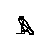
\includegraphics[scale=1.09]{eg/pam}}}
	\DeclareMathOperator{\rDl}{\text{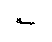
\includegraphics[scale=1.09]{eg/dl}}}
	\DeclareMathOperator{\rSos}{\text{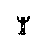
\includegraphics[scale=1.09]{eg/sos}}}

\begin{document}

   \newcommand{\enumsep}{\vspace{-2.8mm}
   		\begin{enumerate}[itemsep=0.4mm,leftmargin=2.5mm]}

\begin{center}
	{\Large Домашнее задание 14. R-Вычислимость и рекурсивность.}

	{\it (7 декабря\ \(\to\)\ 14 декабря)}
\end{center}

\begin{enumerate}

	\item Пусть \(\rOp\lr*{a}\) означает, что $a$ является кодом некоторого оператора; \(\rPr\lr*{a}\) означает, что $a$ является кодом некоторой программы; и \(\rRe\lr*{i,a}\) означает, что $a$ является кодом некоторой программы, содержащей переменную $r_i$.

Докажите, что предикаты \(\rOp\), \(\rPr\) и \(\rRe\) рекурсивны.

	\item Пусть \(\rDl\lr*{a}=l+1\), если $a$ является кодом некоторой программы длины $l+1$, и \(\rDl\lr*{a}=0\), если $a$ не является кодом программы. 

	Пусть \(\rPam\lr*{a}\) равно памяти программы с кодом $a$, если $a$ является кодом некоторой программы, и \(\rPam\lr*{a} = 0\) в противном случае. 

Пусть \(\rSos\lr*{a,x_0,\ldots,x_n,t}=\langle s\rangle\), если $a$ является кодом программы $P$ и $s$ --- состояние $P$ в момент $t$ при вычислении $\varphi_P(\bar{x})$, и сос$(a,x_0,\ldots,x_n,t)=0$, если $a$ не является кодом программы. 
\medskip

Докажите, что функции \(\rDl\), \(\rPam\), и \(\rSos\) рекурсивны.

	\item Докажите, что функция на множестве натуральных чисел R-вычислима тогда и только тогда, когда она рекурсивна. (Учтите все технические детали, которые были пропущены на лекции.)

	Докажите, что частичная функция на множестве натуральных чисел R-вычислима тогда и только тогда, когда она рекурсивна.

	\item Пусть $g$~— произвольная функция на $\mathbb{N}$. Функция $f$ {\it рекусивна относительно} $g$ (символически, $f\leq_Tg$), если $f$ получается из $g,\: +,\: \cdot,\: \chi_<,\: I^n_k$ последовательными применениями суперпозиции и минимизации.

Функция $f$ {\it R-вычислима относительно} $g$, если существует вычисляющая ее программа с оракулом $g$: формально, оператор присваивания может принимать ещё вид \(r_i \coloneqq g(r_i)\).

Докажите равносильность этих двух определений: функция рекурсивна относительно \(g\) тогда и только тогда, когда она R-вычислима относительно \(g\).

	\item Пусть $\varphi_n=\varphi^{(1)}_P$, если $n$ является кодом программы $P$ и $\varphi_n=\emptyset$, если $n$ не является кодом программы. Тогда $\varphi$ --- нумерация всех рекурсивных частичных функций, а $W_n=dom(\varphi_n)$ --- нумерация всех рекурсивно перечислимо множеств.

Докажите, что частичная функция $(n,x)\mapsto\varphi_n(x)$ рекурсивна, а множество $\{n\mid n\in W_n\}$ рекурсивно перечислимо, но не рекурсивно.

\end{enumerate}

\end{document}
